
\documentclass[ms.tex]{subfiles} 
\begin{document} 

\section{Methods} 
\label{sec:methods} 

\begin{itemize} 
	\item Since we wish to test the impact of various assumptions about 
	nucleosynthetic yields while taking into account stellar migration, 
	multi-zone chemical evolution models are the ideal experiments. 
\end{itemize} 

\subsection{The Multi-Zone Chemical Evolution Model} 
\label{sec:methods:multizone} 

\begin{itemize} 
	\item We make use of the Milky Way models of~\citet{Johnson2021}, who 
	originally constructed the model to explore the impact of stellar migration 
	on the observed abundances of oxygen and iron. 
	This model makes use of the~\texttt{Versatile Integrator for Chemical 
	Evolution}~\citep[\vice;][]{Johnson2020, Griffith2021, Johnson2021}, an 
	open-source~\texttt{python} package for~\texttt{Unix} system architectures. 
	Because~\vice~recognizes most elements on the periodic table, computing 
	N abundances with this model is easy. 
	Though we provide a brief summary here, a full breakdown of 
	the~\citet{Johnson2021} model can be found in their~\S~2. 
\end{itemize} 

\subsection{Nucleosynthetic Yields} 
\label{sec:methods:yields} 

\begin{itemize} 
	\item Since we're interested in N and O abundances in the present paper, 
	the relevant nucleosynthetic channels are CCSNe and AGB 
	stars~\citep{Johnson2019}. 
	\citet{Johnson2021} investigated the O and Fe 
	abundances predicted by these models, the relevant sources for which are 
	CCSNe and SNe Ia. 
	Here we simply set the SN Ia yields of N and O to zero, and focus the rest 
	of this section on discussion of their CCSN and AGB star yields. 
\end{itemize} 

\subsubsection{Core Collapse Supernovae} 
\label{sec:methods:yields:ccsn} 

\begin{figure*} 
\centering 
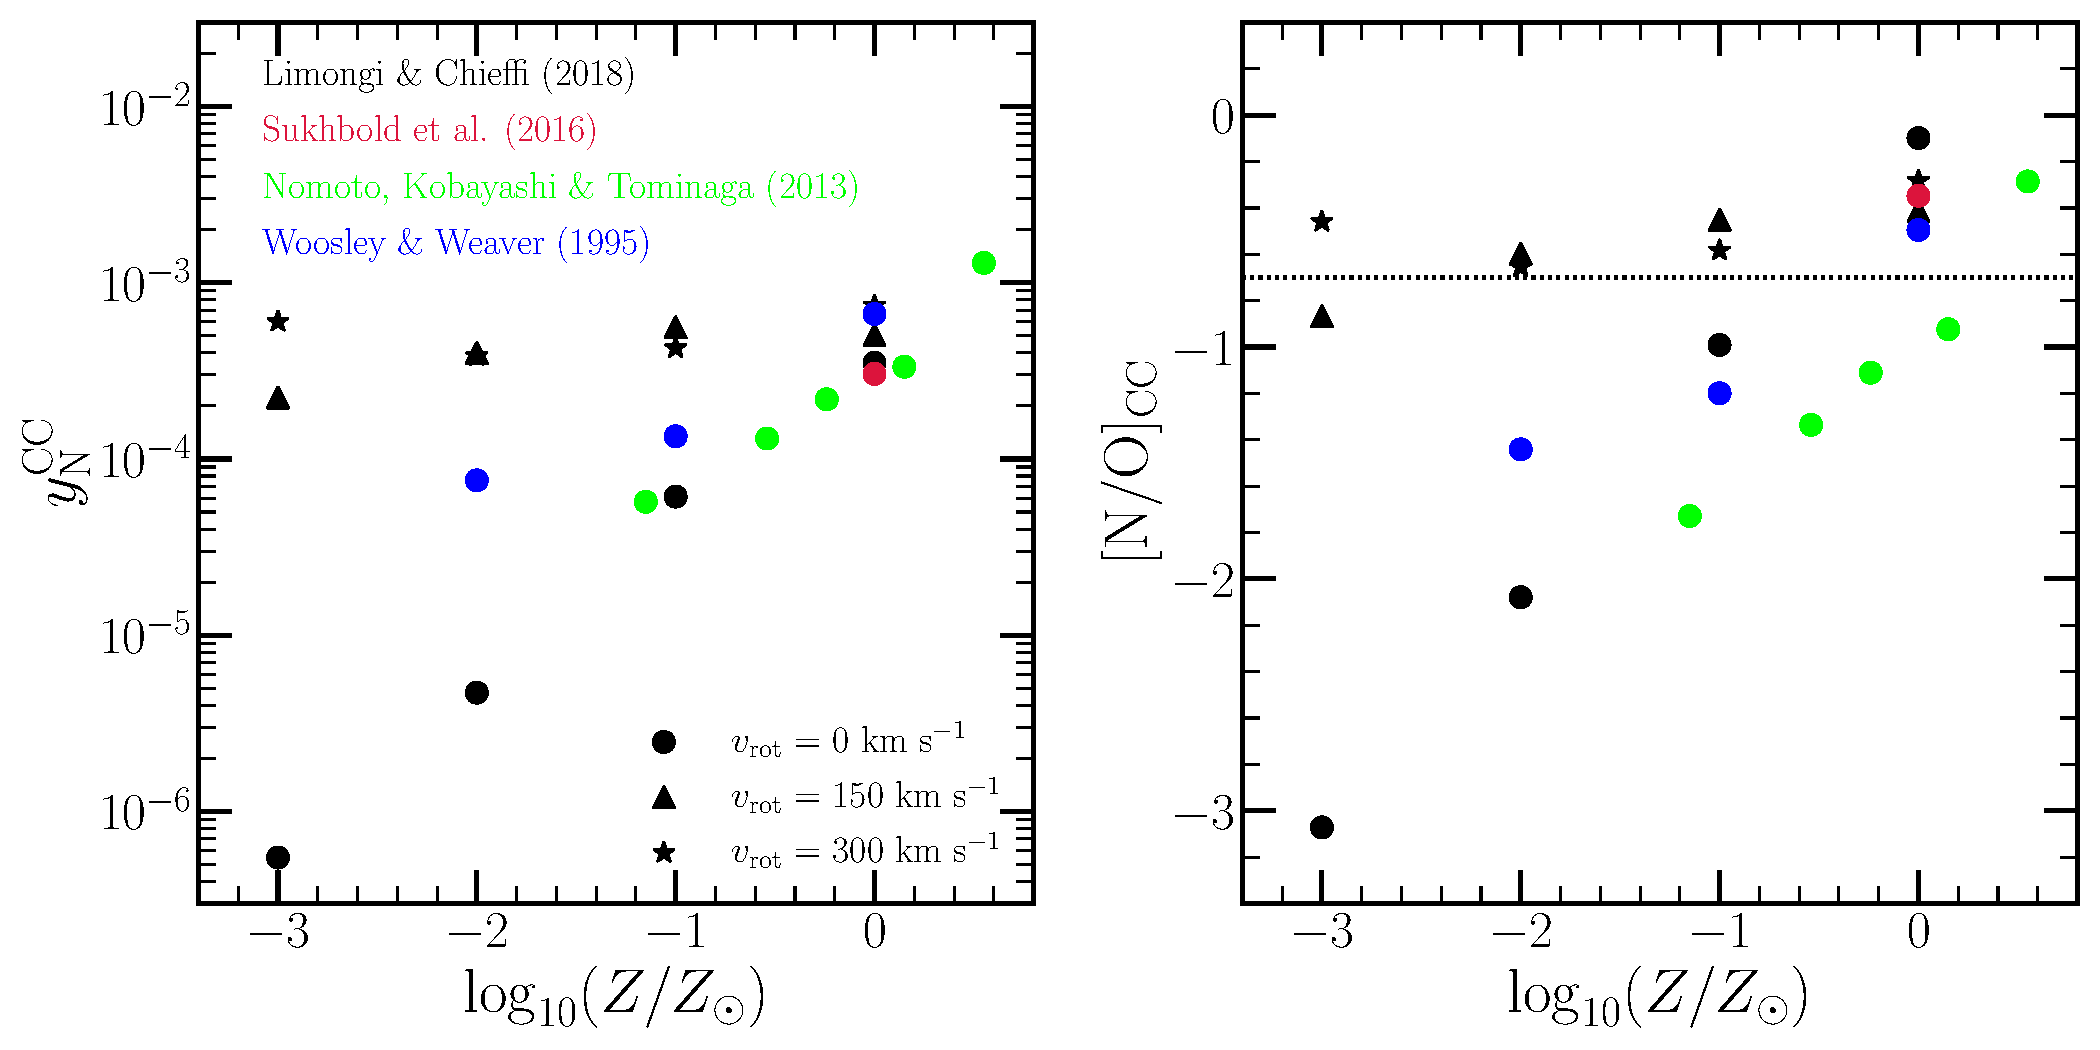
\includegraphics[scale = 0.5]{n_cc_yields.pdf} 
\caption{
\textbf{Left}: IMF-averaged CCSN yields of N calculated 
using~\vice's~\texttt{vice.yields.ccsne.fractional} function with the tables 
published by~\citet[][blue]{Woosley1995},~\citet*[][green]{Nomoto2013}, 
\citet[][red]{Sukhbold2016}, and~\citet[][black]{Limongi2018}. 
All studies report yields for non-rotating progenitors only with the exception 
of~\citet{Limongi2018}, who also report yields for progenitor rotational 
velocities of 150 (triangles) and 300 km/s (stars). 
\textbf{Right}: The~\no~ratio predicted by each of the explosion models in 
the left-hand panel, under the same colour-coding and marker scheme. 
We mark the position of~\no~= $-0.7$ with a black dotted line, the value 
roughly suggested by the observations of low-metallicity systems highlighted in 
Fig.~\ref{fig:no_oh_observed}. 
}
\label{fig:n_cc_yields} 
\end{figure*} 

\newcommand{\subcc}{\ensuremath{_\text{cc}}} 

\begin{itemize} 
	\item For O and Fe, we retain the values of~$y_\text{O}^\text{CC}$ = 0.015 
	and~$y_\text{Fe}^\text{CC}$ = 0.0012 from~\citet{Johnson2021}, who in turn 
	take these values from~\citet{Johnson2020} and~\citet{Weinberg2017}. 
	In~\vice, CCSN nucleosynthetic products are approximated to be produced 
	instantaneously following an episode of star formation; this is a valid 
	approximation due to how short the lives of massive stars are compared to 
	the relevant timescales for GCE. 
	The yield is the constant of proportionality between the CCSN production 
	rate and the SFR: 
	\begin{equation} 
	\dot{M}_\text{X}^\text{CC} = y_\text{X}^\text{CC}\dot{M}_\star. 
	\end{equation} 
	As a consequence of this formulation~$y_\text{X}^\text{CC}$ describes the 
	fraction of a stellar population's initial mass which is processed into 
	some element X and ejected to the ISM via CCSN events 
	(e.g. if~$y_\text{X}^\text{CC}$ = 0.01, a hypothetical 100~\msun~stellar 
	population would produce 1~\msun~of element X). 

	\item At low [O/H]\footnote{
		We follow the standard notation where 
		[X/Y]~$\equiv \log_{10}(X/Y) - \log_{10}(X/Y)_\odot$. 
	}, the mean~\no~is near~$\sim$-0.7. 
	Since the AGB star yields of N are believed to increase with 
	metallicity~\citep{Cristallo2011, Cristallo2015, Ventura2013}, this is 
	likely the regime in which N yields are dominated by CCSN enrichment. 
	Therefore,~\no\subcc~$\approx -0.7$ empirically. 

	\item Based on the definition of the abundance ratio [X/Y], we can relate 
	the CCSN yields of N and O to one another given this result: 
	\begin{subequations}\begin{align} 
	\text{[N/O]}\subcc &= 
	\log_{10}\left(\frac{y_\text{N}^\text{CC}}{y_\text{O}^\text{CC}}\right) - 
	\log_{10}\left(\frac{Z_{\text{N},\odot}}{Z_{\text{O},\odot}}\right) 
	\label{eq:no_cc}
	\\ 
	y_\text{N}^\text{CC} &= 
	y_\text{O}^\text{CC} 10^{\no\subcc} 
	\left(\frac{Z_{\text{N},\odot}}{Z_{\text{O},\odot}}\right), 
	\end{align}\end{subequations} 
	where~$Z_{\text{X},\odot}$ is the abundance by mass of some element X in 
	the sun. 

	\item Taking~$Z_{\text{N},\odot} = 6.91\times10^{-4}$ 
	and~$Z_{\text{O},\odot} = 5.7\times10^{-3}$ based on the solar photospheric 
	abundances of~\citet{Asplund2009} and our value of~$y_\text{O}^\text{CC}$ = 
	0.015 yields~$y_\text{N}^\text{CC} = 3.6\times10^{-4}$, which we adopt as 
	our fiducial CCSN yield of N. 

	\item Can we understand this value with theoretically predicted N yields? 
	To address this, we compute IMF-averaged net yields of N using~\vice's 
	\texttt{vice.yields.ccsne.fractional} function assuming 
	a~\citet{Kroupa2001} IMF; for details, we refer readers to~\S~4 
	of~\citet{Griffith2021} and the~\vice~science documentation.\footnote{
		\url{https://vice-astro.readthedocs.io/en/latest/science_documentation/yields/index.html} 
	} 
	The left panel of Fig.~\ref{fig:n_cc_yields} plots the results as a 
	function of progenitor metallicity predicted by the~\citet{Woosley1995}, 
	\citet{Nomoto2013},~\citet{Sukhbold2016}, and~\citet{Limongi2018} tables. 

	% \item The left panel of Fig.~\ref{fig:n_cc_yields} plots the IMF-averaged 
	% CCSN yields of N as predicted by~\citet{Woosley1995},~\citet{Nomoto2013}, 
	% \citet{Sukhbold2016}, and~\citet{Limongi2018}. 
	%  using~\vice's~\texttt{vice.yields.ccsne.fractional} 
	% function assuming a~\citet{Kroupa2001} IMF 

	% These values, computed using~\vice's~\texttt{vice.yields.ccsne.fractional} 
	% function, describe the fractional net yield of an element X given by: 
	% \begin{equation} 
	% y_\text{X}^\text{CC} = \ddfrac{
	% 	\int_{8~\msun}^u (E(m)m_\text{X} + w_\text{X} - Z_\text{X,prog}m)
	% 	\frac{dN}{dm} dm 
	% }{
	% 	\int_l^u m\frac{dN}{dm} dm 
	% }, 
	% \end{equation} 
	% where~$m_\text{X}$ is the total mass of the element X in the supernova 
	% ejecta of a star of initial mass~$m$,~$w_\text{X}$ is the wind yield, 
	% $Z_\text{X,prog}$ is the initial abundance by mass of the element X in the 
	% star,~$E(m)$ is a function describing whether or not the star explodes as a 
	% supernova, and~$dN/dm$ is the adopted stellar IMF, for which we take 
	% the~\citet{Kroupa2001} form throughout this paper. 
	% These yields are fractional in that they're in units of the progenitor 
	% stellar population's mass (i.e. if~$y_\text{X}^\text{CC}$ = 0.01, a 
	% hypothetical 100~\msun~cluster would produce 1~\msun of X), and they're net 
	% rather than gross in that they quantify only the newly produced mass. 
	% The lower bound of the integral in the numerator, taken to be 8~\msun~here, 
	% simply corresponds to the minimum initial mass for a CCSN event, where the 
	% remaining bounds are simply the lower and upper mass bounds of star 
	% formation, for which we adopt~$l = 0.08$~\msun and~$u = 100$~\msun. 
	% For further details, we refer readers to~\S~4 of~\citet{Griffith2021} and 
	% the~\vice~science docuementation.\footnote{
	% 	\url{https://vice-astro.readthedocs.io/en/latest/science_documentation/yields/index.html} 
	% } 

	\item Only~\citet{Limongi2018} report yields for progenitors with a 
	non-zero rotational velocity, and these are the only values consistent 
	with~$y_\text{N}^\text{CC} = 3.6\times10^{-4}$ at low metallicity. 
	For non-rotating progentiors, every study investigated here can reproduce 
	approximately this value at solar metallicity only, with the predictions at 
	lower~$Z$ falling short of the empirical value, in some cases by orders of 
	magnitude. 

	\item It is unsurprising that~$y_\text{N}^\text{CC}$ is so dependent on the 
	rotational velocity at low metallicity. 
	$y_\text{N}^\text{CC}$ is itself highly uncertain at 
	low~$Z$~\citep{Heger2010}, but most of the N production in CCSN progenitors 
	occurs via the CNO cycle processing C and O isotopes into~\Nfourteen. 
	With few C and O seed nuclei at low~$Z$, production of~\Nfourteen~is 
	difficult. 
	Rotationally induced mixing, also a highly uncertain process 
	\citep{Frischknecht2016}, could transport newly produced C and O into the 
	hydrogen burning shell of the CCSN progenitor~\citep[see discussion 
	in~\S~4.2 of][]{Andrews2017}. For this reason, N yields at low metallicity 
	are highly sensitive to the assumptions about mixing. 

	\item In the right-hand panel of Fig.~\ref{fig:n_cc_yields}, we make use of 
	equation~\refp{eq:no_cc} to compare the~\no~ratios predicted by these 
	studies; the horizontal black dashed line denotes~\no\subcc~$= -0.07$, the 
	empirical value taken from Fig.~\ref{fig:no_oh_observed}. 
	The fact that the points follow similar trends between the two panels is a 
	consequence of the fact that these studies predict metallicity-independent 
	O yields~\citep{Griffith2021}. 

	\item Again, only the rotating models of~\citet{Limongi2018} are able to 
	reproduce this value at low metallicity. 
	At solar metallicity the supernova models predict a higher~\no\subcc, but 
	our value of~\no\subcc~is taken at low metallicity, so that is the 
	most relevant comparison. 
\end{itemize} 

\subsubsection{Asymptotic Giant Branch Stars} 
\label{sec:methods:yields:agb} 

\begin{figure*} 
\centering 
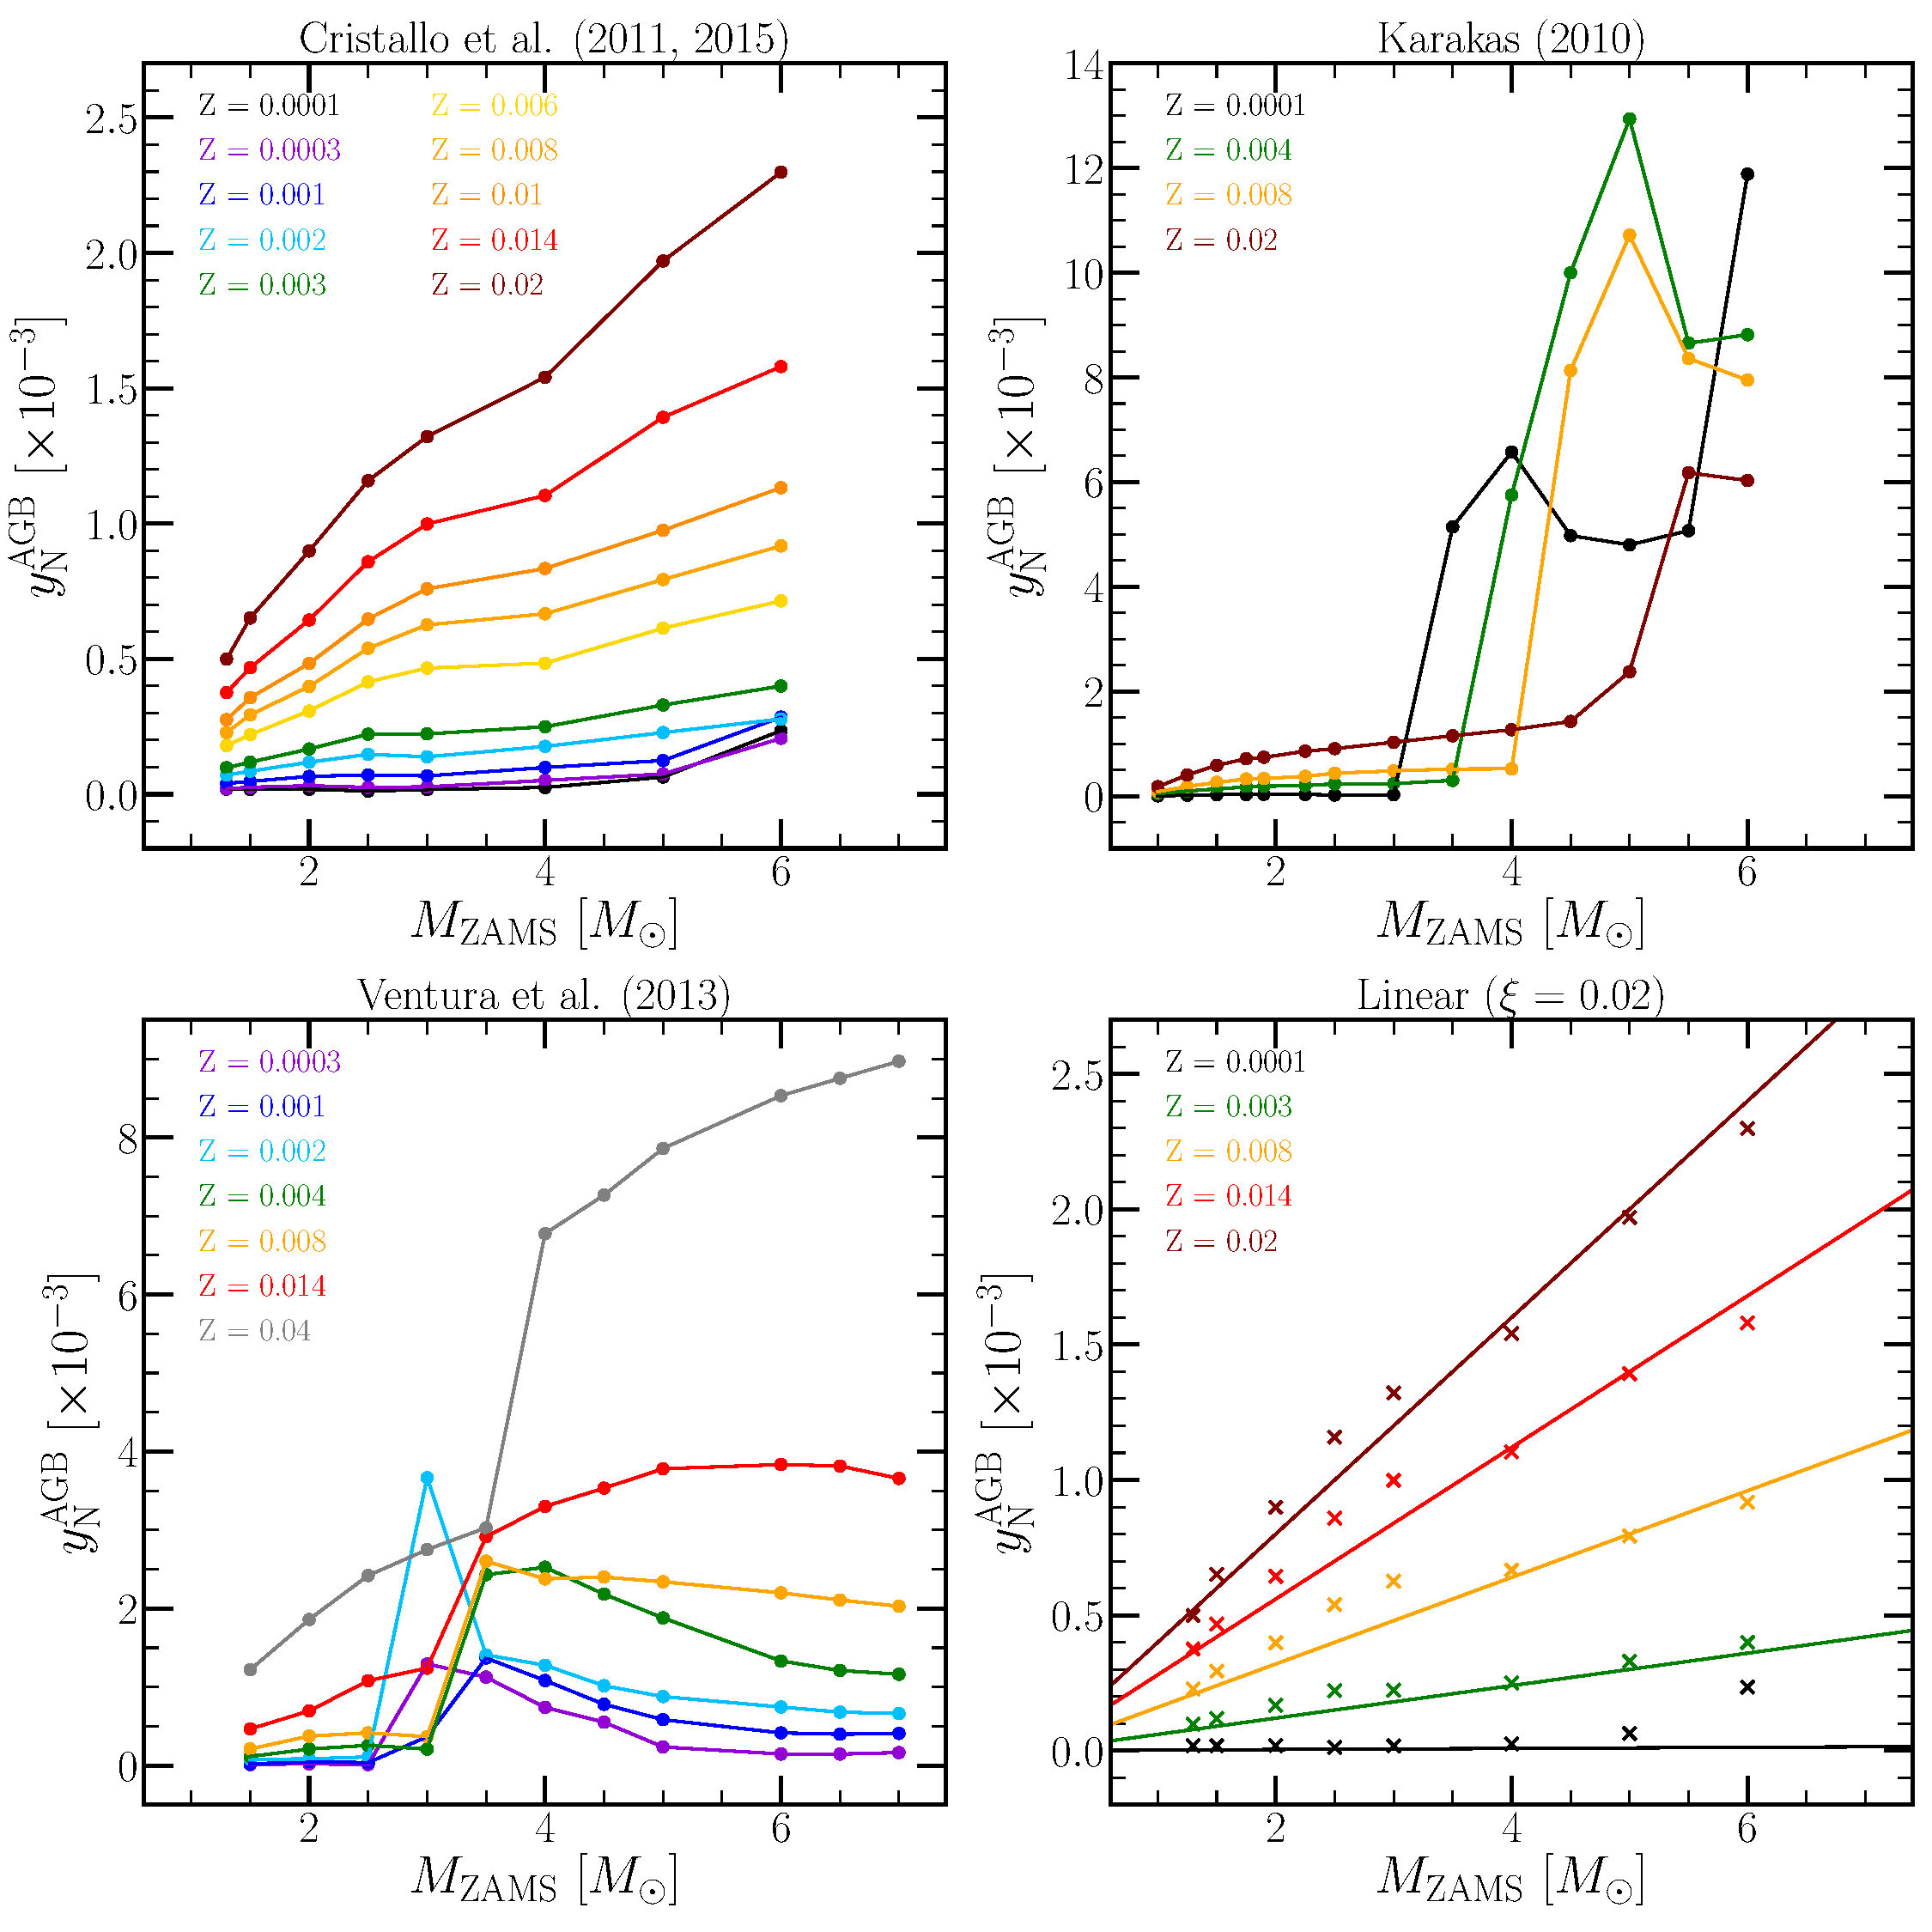
\includegraphics[scale = 0.33]{agb_yield_models.pdf} 
\caption{
The fractional yields of N from AGB stars~$y_\text{N}^\text{AGB}$ as a function 
of progenitor ZAMS mass and birth metallicity~$Z$ as reported 
by~\citet{Karakas2010} (upper left),~\citet{Karakas2016} and~\citet{Karakas2018} 
(upper middle),~\citet{Cristallo2011, Cristallo2015} (lower left), 
and~\citet{Ventura2013} (lower middle). 
In the lower right panel, we show the yields predicted by our linear model 
(colored lines; see discussion in~\S~X) in comparison to 
the~\citet{Cristallo2011, Cristallo2015} predictions (colored X's). 
}
\label{fig:agb_yield_models} 
\end{figure*} 

\begin{itemize} 
	\item In the present paper, we're interested in the question of how 
	well the ``off the shelf'' AGB star yield models for N can reproduce the 
	observed [N/O]-[O/H] relation. 

	\item As previously discussed, the majority of nitrogen production occurs 
	through the CNO cycle, the slowest component of which is the 
	\Nfourteen(p,$\gamma$)\Ofifteen reaction which produces a bottleneck, 
	effectively turning all of the different C, N, and O isotopes 
	into~\Nfourteen. 

	\item Similar to the CCSN yields discussed 
	in~\S~\ref{sec:methods:yields:ccsn}, these are defined as fractional net 
	yields in that they quantify only the newly produced N in the AGB star 
	ejecta in units of its ZAMS mass. 
	For a yield~$y_\text{N}^\text{AGB}(M_\star, Z_\star)$, the actual mass 
	yield is then given by~$M_\star y_\text{N}^\text{AGB}(M_\star, Z_\star)$. 

	\item We make use of tables that are built into~\vice, two of which are new 
	to this study and are included in its latest release. 
	\begin{itemize} 
		\item The default set of yields, published in~\citet{Cristallo2011, 
		Cristallo2015} is plotted in the lower left panel of 
		Fig.~\ref{fig:agb_yield_models}. 
		This is the most comprehensive set of yields in~\vice~in that it 
		includes tables for all elements built into the code and is sampled at 
		the most metallicities. 

		\item The~\citet{Karakas2010} set of yields, also previously built 
		into~\vice, is plotted in the upper left panel. 

		\item We obtain the yields from~\citet{Ventura2013}, which are new 
		to~\vice, and plot them in the lower middle panel. 

		\item We combine the yields published in~\citet{Karakas2016} at~$Z$ = 
		0.007, 0.014, and 0.03 with those published in~\citet{Karakas2018} 
		at~$Z$ = 0.0028 and build them into~\vice~as well. 
		Although there are yields published in both~\citet{Karakas2016} 
		and~\citet{Karakas2018} in this table, we hereafter refer to this set 
		as the~\citet{Karakas2016} set for simplicity. 
		We plot them in the upper middle panel of 
		Fig.~\ref{fig:agb_yield_models}. 
	\end{itemize} 

	\item \vice~also allows users to construct their own functions of 
	progenitor mass and metallicity to describe the AGB star yield. 
	As an additional test, we construct a model in which the yield is linearly 
	proportional to both of them according to: 
	\begin{equation} 
	y_\text{N}^\text{AGB} = \xi\left(\frac{M}{M_\odot}\right) 
	\left(\frac{Z}{Z_\odot}\right) 
	\label{eq:linear_yield} 
	\end{equation} 
	We illustrate this model in the lower right panel of 
	Fig.~\ref{fig:agb_yield_models} for~$\xi = 3\times10^{-4}$. 
	We compare this model to the~\citet{Cristallo2011, Cristallo2015} yields by 
	including the colored X's on this panel. 
	In general, the two yield models agree rather well. 

	\item Despite reporting values of the same physical quantities, the N 
	yields reported by each of these studies show substantial differences 
	between one another. 
	Unfortunately, a direct comparison between AGB star yield tables is 
	difficult, because each study employs different assumptions for mass loss, 
	convection and covective boundaries within the star, and nuclear reaction 
	networks, all of which have a significant impact on stellar evolution and 
	consequently the predicted abundances. 
	However, the two most important physical processes in determining AGB star 
	yields of all the CNO species is third dredge up (TDU) and hot bottom 
	burning (HBB), and some of the differences between these yield sets can be 
	understood through the interaction between the two. 
	\begin{itemize} 
		\item TDU refers to the repeated penetrations of the convective 
		envelope into the hydrogen depleted core during the thermal pulses 
		associated with AGB star evolution. 
		This process doesn't affect N abundances much, but replenishes the 
		outer layers of the star with C and O. 
		In low mass AGB stars, the main source of free neutrons is the 
		\Cthirteen($\alpha$,n)\Osixteen~reaction, which can occur at 
		substantial rates when C is mixed with the He-rich shell during each 
		TDU episode. 

		\item HBB refers to the activation of proton captures at the base of 
		the convective envelope, which activates the CNO cycle, producing large 
		amounts of~\Nfourteen. HBB requires a higher mass AGB star progenitor 
		($\sim$4 - 5~\msun at Z$_\odot$) than TDU ($\sim$2 - 2.5~\msun at 
		Z$_\odot$), but the minimum mass for both decreases at lower 
		metallicity. 

		\item The most efficient N production occurs when both TDU and HBB 
		occur within an AGB star, because each replenishment of C and O 
		isotopes from the core adds new seed nuclei for the CNO cycle when HBB 
		is active. 
		This is the reason for the substantial N production 
		above~$\sim$4~\msun in the~\citet{Karakas2010} and~\citet{Karakas2016} 
		models; in both yield sets, every star that experiences HBB also 
		experiences TDU. 
		Both TDU and HBB are more efficient at low metallicity~\citep[see 
		discussion in][]{Ventura2013}. 
		In the case of TDU, each penetration of the convective envelope into 
		the H-depleted core is deeper because of the lower opacity. 
		For HBB, the base of the convective envelope is hotter, increasing the 
		rate of nuclear reactions relative to the higher~$Z$ models. 
		Though some exceptions are evident in Fig.~\ref{fig:agb_yield_models}, 
		as a result of this the highest N yields in the~\citet{Karakas2010} 
		and~\citet{Karakas2016} tables are for the low metallicity stars 
		above~$\sim$4~\msun. 

		\item This same interaction between TDU and HBB is also the reason for 
		the increase in yields in the~\citet{Ventura2013} sample. 
		Unlike~\citet{Karakas2010} and~\citet{Karakas2016}, their models 
		experience both TDU and HBB only near~$\sim$3~\msun. 

		\item Of all of these yields taken from the literature, 
		the~\citet{Cristallo2011, Cristallo2015} sample shows the smoothest 
		dependence on progenitor mass and metallicity. 
		Unfortunately, ascertaining the exact cause of this difference between 
		the other yields explored here is difficult; relative to 
		the~\citet{Karakas2016} yields (see discussion in their~\S~5), 
		the~\citet{Cristallo2011, Cristallo2015} models have more mass loss, 
		a~$\sim$10\% faster triple-$\alpha$ reaction rate, weaker HBB, and 
		fewer thermal pulses overall. 
		The fact that HBB is weaker and fewer TDU episodes are experienced does 
		however lend a qualitative explanation into why 
		the~\citet{Cristallo2011, Cristallo2015} yields are so much smaller 
		than the~\citet{Karakas2010} and~\citet{Karakas2016} yields at higher 
		masses. 
	\end{itemize} 

\end{itemize} 



















\end{document} 
